\documentclass{standalone}
\usepackage{tikz}

\begin{document}

\begin{tikzpicture}[scale=2]
    % Define the sequence length
    \def\sequenceLength{16}
    
    % Draw the x-axis
    \draw[->] (-0.5,0) -- (\sequenceLength+0.5,0);
    
    % Draw the dashed line at elevation zero
    \draw[dashed] (0,-0.3) -- (\sequenceLength+0.5,-0.3);
    
    % Initialize elevation
    \def\elevation{0}
    
    % Loop through each character in the sequence
    \foreach \char [count=\i] in {R,R,R,L,L,R,L,L,L,R,L,R,R} {
        % Update elevation based on the character
        \ifx\R\char
            \def\elevation{\elevation+1}
        \fi
        \ifx\L\char
            \def\elevation{\elevation-1}
        \fi
        
        % Mark the position if elevation is zero
        \ifnum\elevation=0
            \fill (\i-0.5,-0.4) circle (0.1);
        \fi
        
        % Draw the vertical line at the current position
        \draw (\i-0.5,0) -- (\i-0.5,\elevation);
        
        % Label the character above the vertical line
        \node at (\i-0.5,\elevation+0.1) {\char};
    }
    
    % Label the sequence below the x-axis
    \node[below] at (\sequenceLength/2, -0.7) {$UD = (RRRLLRLL)(LLRLRLRR)$};
\end{tikzpicture}

\end{document}